\chapter{Result}
\label{chapter:result}
%\TODO{In this chapter, we will describe the evaluation methodology and experimental results of our system. }
The main contribution of this thesis work is the view-dependent progressive mesh streaming framework on iPad. We have described and illustrated the design and implementation details of our system in previous chapters. In this chapter, we will do some experiment on our system and illustrate the evaluation results.  

\section{Overview}
\label{chapter:result:overview}
Since our framework provides both client and server rendering of progressive mesh, experiments are performed both for client rendering and server rendering scenario. The initial purpose of providing two ways of rendering is to process large models which are not suitable for client rendering, therefore we will different models will be used to test the system's performance in both scenarios. 
\subsection{Models for Test}
\label{chapter:result:overview:modelfortest}
Below is a list of test models: 
\begin{table}
\begin{center}
    \begin{tabular}{|	p{7.5cm}	|	l	|	l	|}
    \hline
    	\textbf{Model Name} 							& \textbf{Num. Vertices} 	& \textbf{Num. Faces}	\\ \hline
	bunny								&2503			&4968		\\ \hline
	bunny\_high							&34834			&69664		\\ \hline
	Armadillo\_mirror						&172974			&345944		\\ \hline
	hand									&210528			&416384		\\ \hline
	angel								&237018			&474048		\\ \hline
	hand\_new							&327323			&654666		\\ \hline
	dragon\_vrip							&437645			&871414		\\ \hline
    \end{tabular}
    \caption{Test models for client rendering.}
    \label{table:modelsclientrendering}
\end{center}
\end{table}

\begin{table}
\begin{center}
    \begin{tabular}{|	p{7.5cm}	|	l	|	l	|}
    \hline	
    	\textbf{Model Name} 						& \textbf{Num. Vertices} 	& \textbf{Num. Faces}	\\ \hline
    	happy\_vrip							&543652			&1087716		\\ \hline
	rolling\_stage\_1.2Mfaces\_edited			&596903			&1192501		\\ \hline
	810\_Red\_circular\_box\_1.4Mtriangles\_clean	&701332			&1402640		\\ \hline
	803\_neptune\_4Mtriangles\_manifold		&2003932			&4007872		\\ \hline
    \end{tabular}
    \caption{Test models for server rendering.}
    \label{table:modelsserverrendering}
\end{center}
\end{table}

\TA{table:modelsclientrendering} lists test models for client rendering and \TA{table:modelsserverrendering} lists test models for server rendering. Models for both situations are sorted according to number of vertices and faces they contain. Here we decide to do server rendering for models with over 1M faces. 

\subsection{Hardware Setup}
%\TODO{This section describes hardwares we used for experiments. }\\
Since our framework is a client-server based application, we will illustration the hardware setup of both client and server side. \\

The \textbf{Client} side application is implemented and deployed on an \textbf{iPad 3rd generation\footnote{\label{ipad3rd}\url{http://support.apple.com/kb/SP647}}}. It has a Dual-core Apple A5X CPU (ARMv7) clocked at 1 GHz, with a system-on-chip quad-core graphics processor and 1 GB RAM. Its operating system is iOS 6.1.3. \\

And the \textbf{Server} side application is implemented and deployed on a \textbf{Macbook} with a Intel Core 2 Duo CPU of 2.4 GHz and 4 GB of DDR3 RAM. The server side operating system is MAC OS X 10.8.3. \\

The \textbf{Network Environment} we experiment in is a 10/100 M WiFi network environment with average roundtrip delay of 30.569 ms

\section{Experiment Results }
\label{section:expresult}
We evaluate our framework separately for server and client rendering scenario. And for each scenario, we measure our framework in three aspects: (1) Transmission Performance, (2) Memory/CPU Usage and (3) Visual Quality. \\

A standard testing process is defined. For each experiment, we will first open the model to test. (As default it will be put in the center of screen. ) Next we start the streaming process until maximum LOD is reached. And then we rotate to the back side and zoom-in to the center-part of the model. The test ends until maximum LOD is reached in current viewing situation. In the following sections we will illustrate the evaluation results of our experiments. 

\subsection{Client Rendering Evaluation}
\label{section:clienteva}
The client rendering evaluation experiments are performed on the models listed in \TA{table:modelsclientrendering}. 
\subsubsection{Transmission Performance}
\label{section:clienttransperf}
\begin{figure}[htb]
	\centering
	
	\begin{pdfpic}
\psline[linewidth=0.05cm,arrowsize=0.05291667cm 2.32,arrowlength=1.4,arrowinset=0.4]{->}(0.38910156,3.9910352)(0.38910156,-4.508965)
\usefont{T1}{ptm}{m}{n}
\rput(2.1228712,4.396035){Client}
\usefont{T1}{ptm}{m}{n}
\rput(5.5489354,4.396035){Server}
\psline[linewidth=0.02cm,linestyle=dashed,dash=0.16cm 0.16cm](2.0891016,4.1910353)(2.0891016,-4.508965)
\psline[linewidth=0.02cm,linestyle=dashed,dash=0.16cm 0.16cm](5.589102,4.1910353)(5.589102,-4.508965)
\usefont{T1}{ptm}{m}{n}
\rput{-90.0}(0.3924024,7.245801){\rput(3.7567968,3.651035){\Huge ...}}
\psline[linewidth=0.04cm,arrowsize=0.05291667cm 2.0,arrowlength=1.4,arrowinset=0.4]{->}(2.3891015,2.5910351)(5.2891016,2.0910351)
\usefont{T1}{ptm}{m}{n}
\rput{-8.649829}(-0.34278482,0.62180525){\rput(3.9170704,2.5960352){SyncViewingParam}}
\psline[linewidth=0.04cm,arrowsize=0.05291667cm 2.0,arrowlength=1.4,arrowinset=0.4]{<-}(2.5293014,0.5025208)(5.248902,1.2795495)
\usefont{T1}{ptm}{m}{n}
\rput{16.396927}(0.4885742,-1.0360752){\rput(3.8367383,1.1960351){VsplitStream}}
\psframe[linewidth=0.04,dimen=outer,fillstyle=solid](5.7891016,2.0910351)(5.3891015,1.1910352)
\usefont{T1}{ptm}{m}{n}
\rput(6.6628613,1.6960351){Processing}
\psframe[linewidth=0.04,dimen=outer,fillstyle=solid](2.2891016,0.29103515)(1.8891015,-0.60896486)
\usefont{T1}{ptm}{m}{n}
\rput(3.5271094,-0.10396484){Refine&Render}
\psframe[linewidth=0.04,dimen=outer,fillstyle=solid](2.2891016,-1.1089648)(1.8891015,-2.4089649)
\usefont{T1}{ptm}{m}{n}
\rput(3.4667382,-1.4039649){ViewingParam}
\psline[linewidth=0.05cm,arrowsize=0.05291667cm 2.32,arrowlength=1.4,arrowinset=0.4]{->}(2.0891016,-0.60896486)(2.0891016,-1.1089648)
\usefont{T1}{ptm}{m}{n}
\rput(3.0408204,-1.7039648){Decrease}
\psline[linewidth=0.04cm,arrowsize=0.05291667cm 2.0,arrowlength=1.4,arrowinset=0.4]{->}(2.2891016,-2.2089648)(5.4891014,-2.8089647)
\usefont{T1}{ptm}{m}{n}
\rput{-8.649829}(0.45317224,0.5464833){\rput(3.8170702,-2.703965){SyncViewingParam}}
\psframe[linewidth=0.04,dimen=outer,fillstyle=solid](5.7891016,-2.7089648)(5.3891015,-3.608965)
\usefont{T1}{ptm}{m}{n}
\rput{-90.0}(7.1924024,0.44580078){\rput(3.7567968,-3.148965){\Huge ...}}
\usefont{T1}{ptm}{m}{n}
\rput(0.35844725,4.396035){Time}
\usefont{T1}{ptm}{m}{n}
\rput(9.480206,1.4960351){Elapsed Time}
\psline[linewidth=0.04cm,arrowsize=0.05291667cm 2.0,arrowlength=1.4,arrowinset=0.4]{->}(7.7891016,0.99103516)(8.389102,1.3910352)
\usefont{T1}{ptm}{m}{n}
\rput{-90.0}(8.092402,-0.45419908){\rput(3.7567968,-4.048965){\Huge ...}}
\psframe[linewidth=0.04,dimen=outer,fillstyle=solid](2.2891016,3.5910351)(1.8891015,2.2910352)
\psframe[linewidth=0.05,linestyle=dashed,dash=0.16cm 0.16cm,framearc=0.25,dimen=outer](7.6891017,3.1910353)(1.3891015,-0.9089649)

	\end{pdfpic} 
	\caption{Client Rendering Transmission Elapsed Time Illustration}
	\label{fig:clientrndtransillu}

\end{figure}
\begin{figure}
\centering
\subfigure[b][Data Transmission. X Axis: time (second), Y Axis: Data (KB).]{
	\centering
	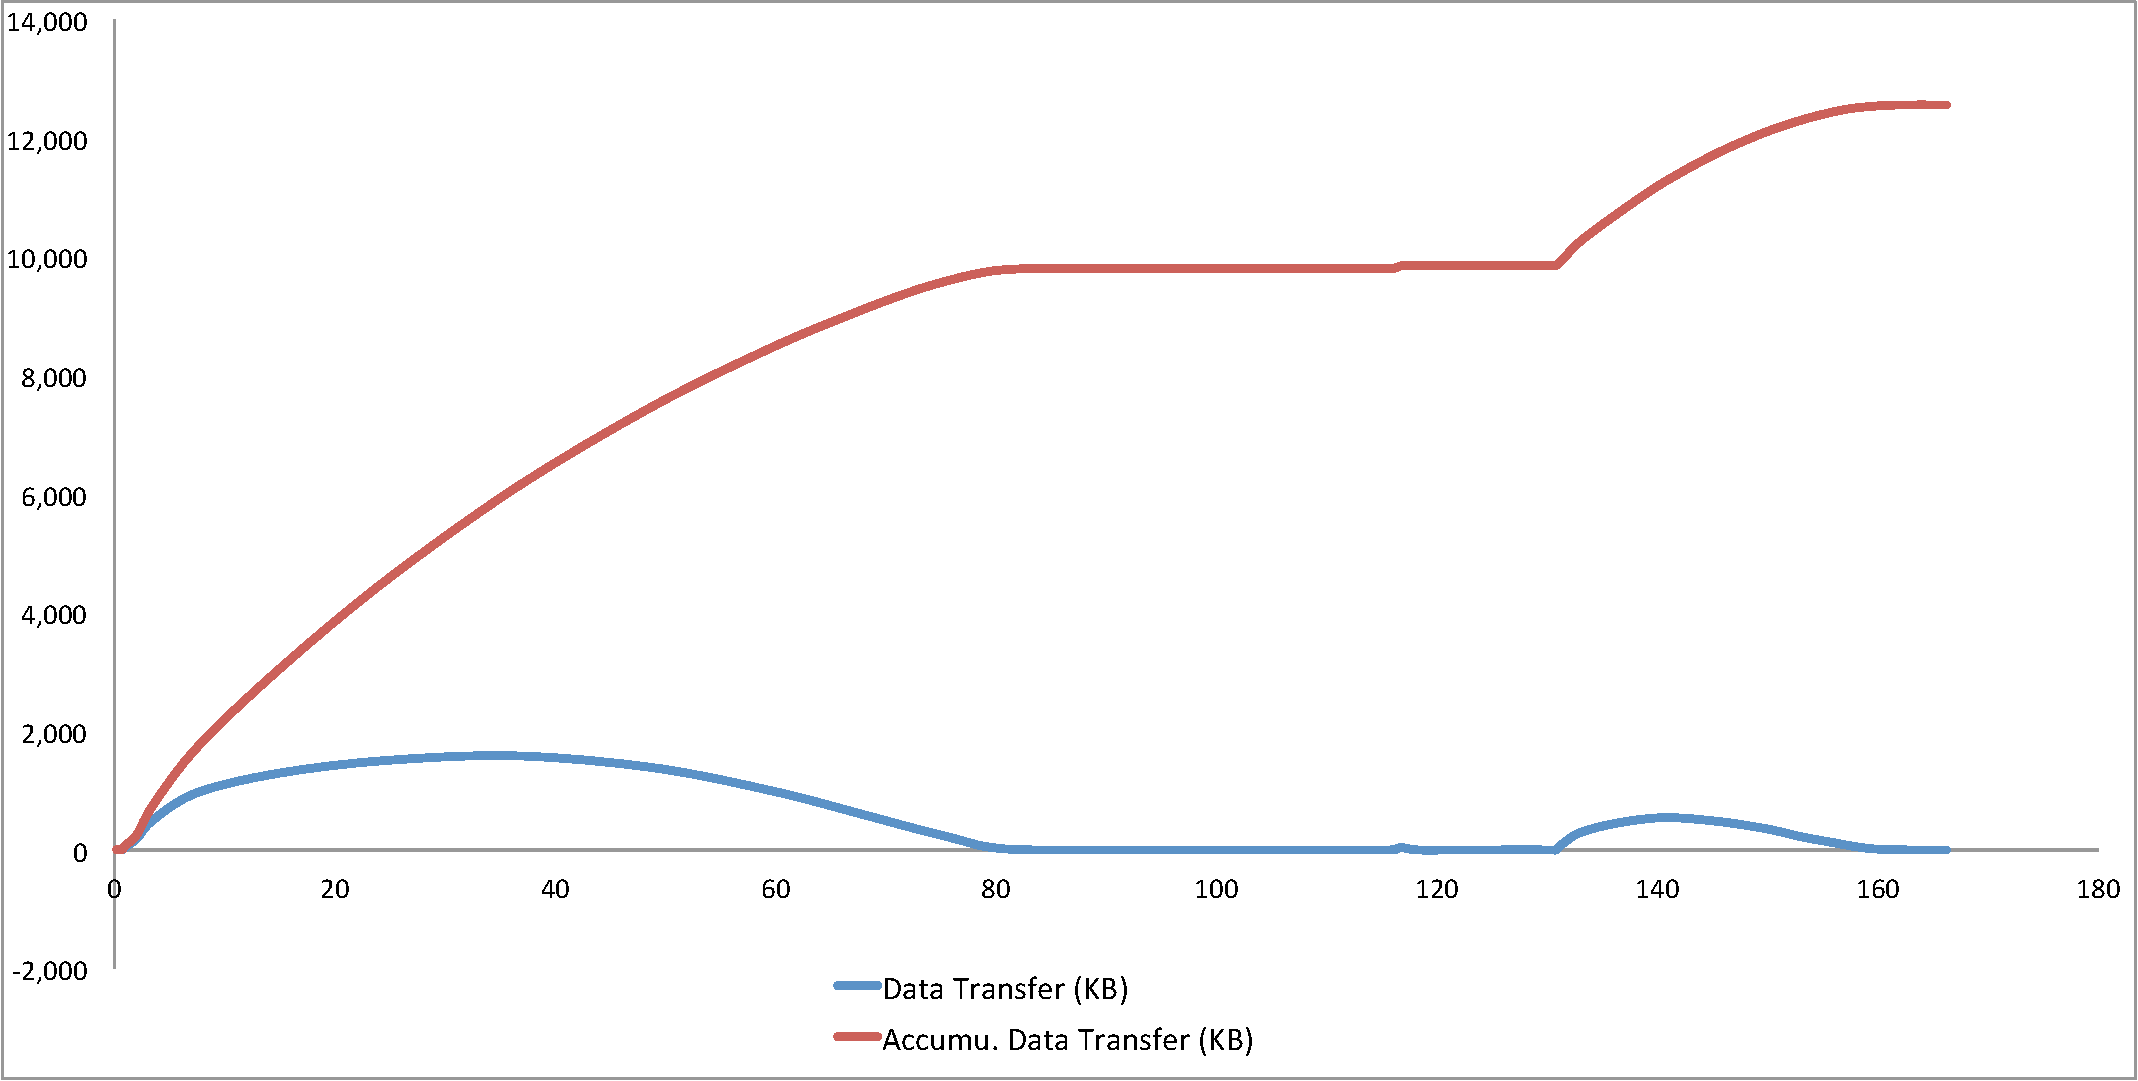
\includegraphics[width =\textwidth] {results/hand_trans_perf.pdf}
	\label{fig:hand_trans_perf_data}
}
\subfigure[b][Elapsed Time of each Viewing Parameter Synchronization. X Axis: Sync Request, Y Axis: Elapsed Time (second)]{
	\centering
	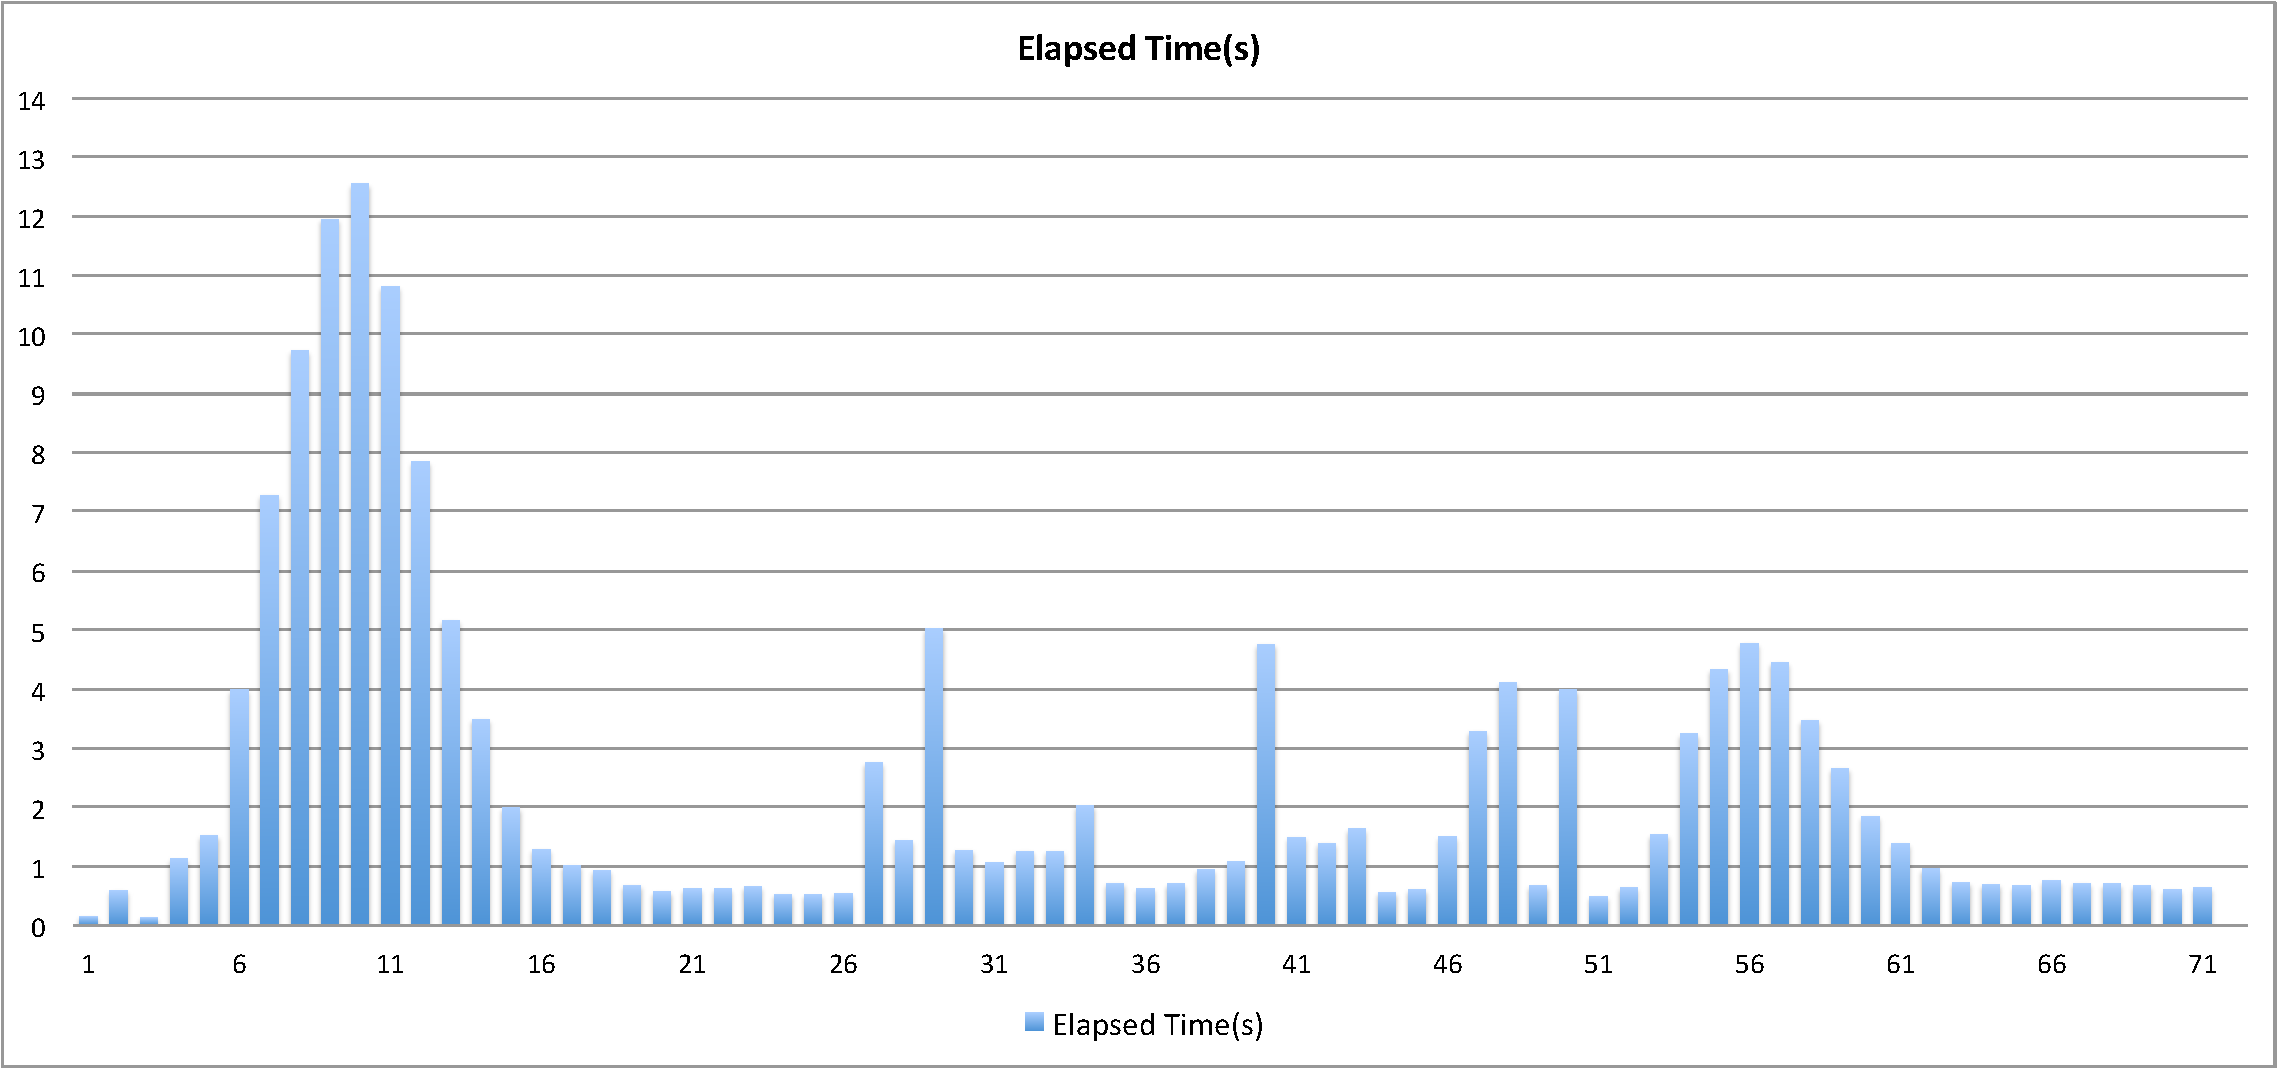
\includegraphics[width =\textwidth] {results/hand_trans_perf_elapsed_time.pdf}
	\label{fig:hand_trans_perf_elapsedtime}
}
\label{fig:hand_trans_perf}
\caption{Client Rendering Data Transmission Performance of Model "hand"}
\end{figure}

\begin{figure}
\centering
\subfigure[b][Data Transmission. X Axis: time (second), Y Axis: Data (KB).]{
	\centering
	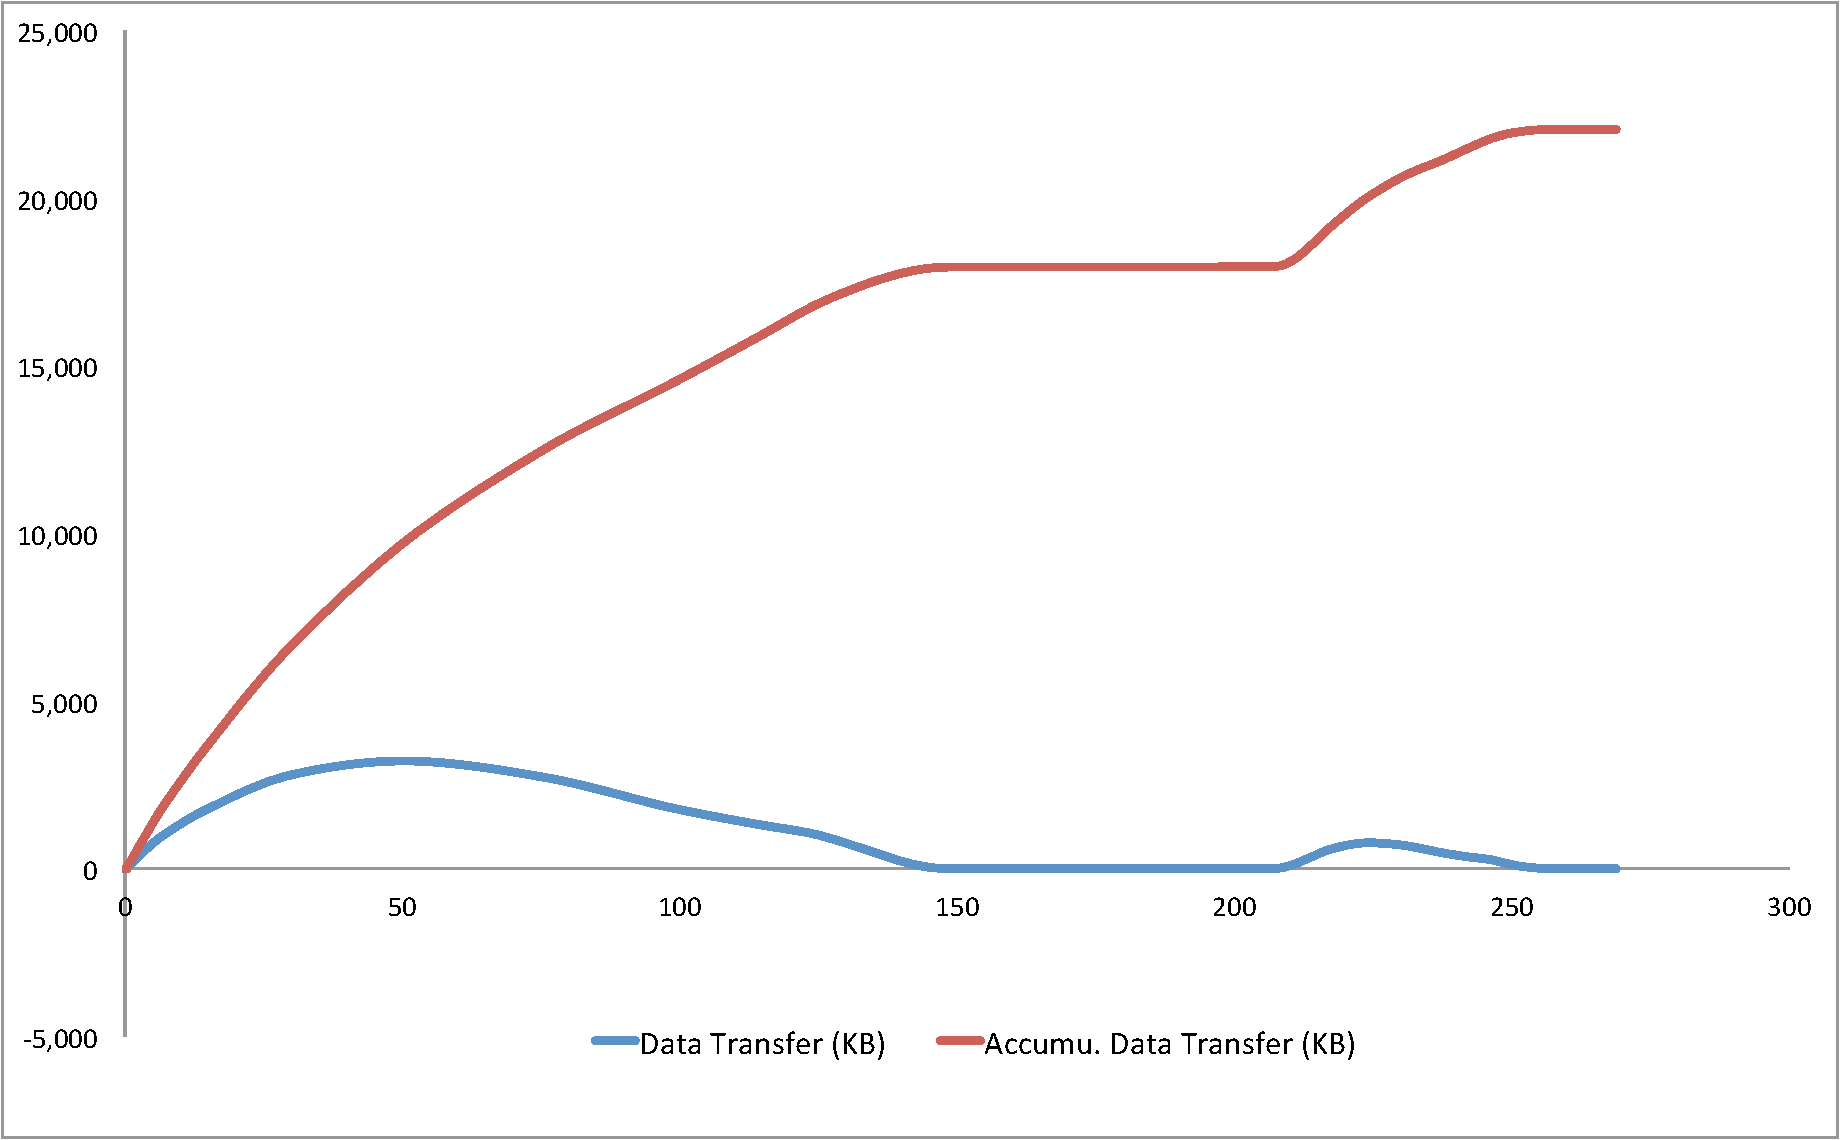
\includegraphics[width =\textwidth] {results/dragon_vrip_trans_perf.pdf}
	\label{fig:dragon_vrip_trans_perf_data}
}
\subfigure[b][Elapsed Time of each Viewing Parameter Synchronization. X Axis: Sync Request, Y Axis: Elapsed Time (second)]{
	\centering
	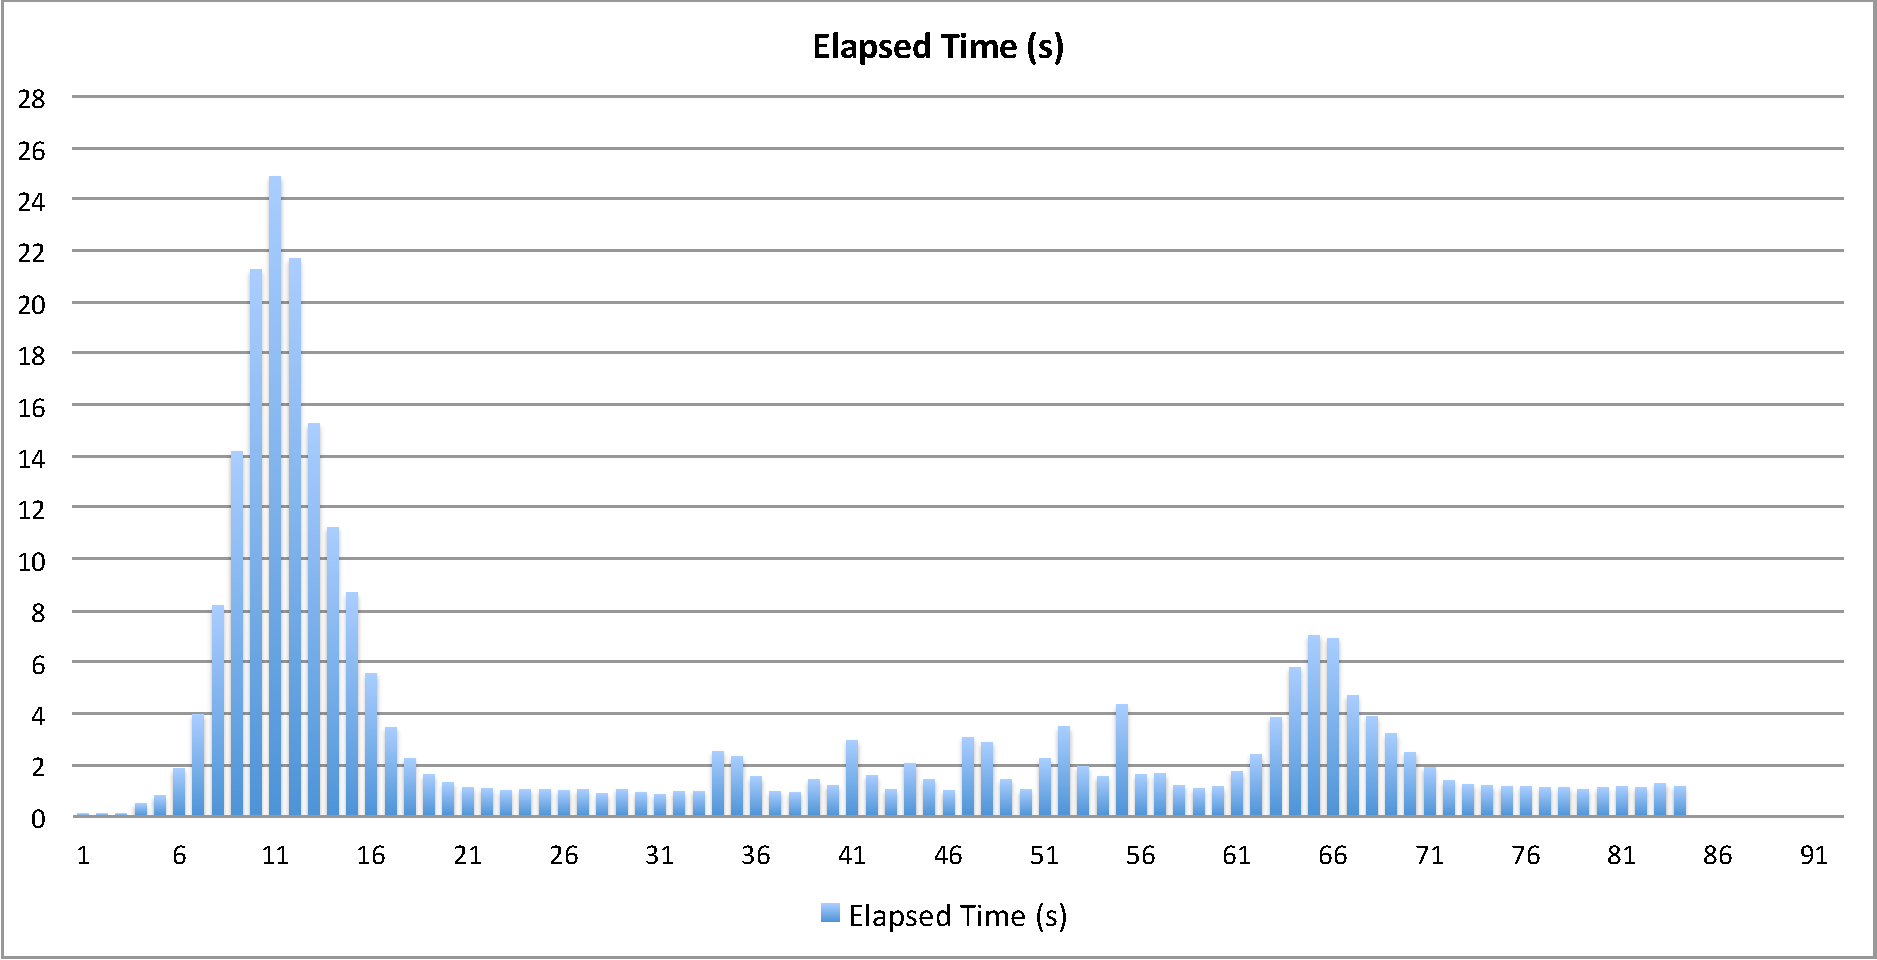
\includegraphics[width =\textwidth] {results/dragon_vrip_trans_perf_elapsed_time.pdf}
	\label{fig:dragon_vrip_trans_perf_elapsedtime}
}
\label{fig:dragon_vrip_trans_perf}
\caption{Client Rendering Data Transmission Performance of Model "dragon\_vrip"}
\end{figure}
Recall the transmission process in the situation of client rendering. When a connection is established and there is no more user interaction on client's screen, the client application will repeatedly reduce the screen error tolerance by half and send the viewing  parameter with updated screen error tolerance to server for new $vsplit$ packets. Then $vsplit$ packets corresponding to current viewing parameter are transmitted to client and the client will perform refinement operation on current mesh. Once the refinement is finished, if there's no more user interaction,  the client will continue to decrease the screen error tolerance and perform the process again until current possible maximum LOD is reached. Therefore, we collect the elapsed time and $vsplit$ packet's size for each viewing parameter synchronization and response process. \FG{fig:clientrndtransillu} illustrates each sampled elapsed time interval. \\

\FGp{fig:hand_trans_perf_data} shows the data transmission performance experiment we performed on model "hand" (See \TAp{table:modelsclientrendering}). The X axis denotes the time passed and the Y axis denotes the data amount in the unit of KB. The blue curve illustrates the data transfer amount upon each viewing parameter synchronization request. And the red curve illustrates the accumulative data transfer amount over the time. It can be discovered that the major data transmission occurs between 0~80 seconds and 130~160 seconds. It is easy to explain: in the first 80 seconds we are streaming from the initial view of the model. And next crest reflects the rotation of view and the streaming process of model's back side geometry. During 80~130 seconds we are interacting with the model to adjust it to the second viewing angle and scale. From \FGp{fig:hand_trans_perf_data} we can also get the time of streaming from base mesh to highest LOD with maximum details for a specific viewing parameter with the model "hand". For the initial one it costs about 80 seconds. And for the second one it costs about 30 seconds. The reason why this time is decreasing is that in the second phase we are viewing (and zooming into) a small area of the model's back center and it naturally contains less detail to refine. \\

\FGp{fig:hand_trans_perf_elapsedtime} shows the elapsed time for each viewing parameter sync request of the experiment on model "hand". The elapsed time includes network transmission time and client-side refine\&render time. Naturally it has similar trend of the blue line in \FGp{fig:hand_trans_perf_data}.





\subsubsection{Memory/CPU Usage}
\label{section:clientmemcpuusage}

\begin{figure}
\centering
\subfigure[b][CPU Usage]{
	\centering
	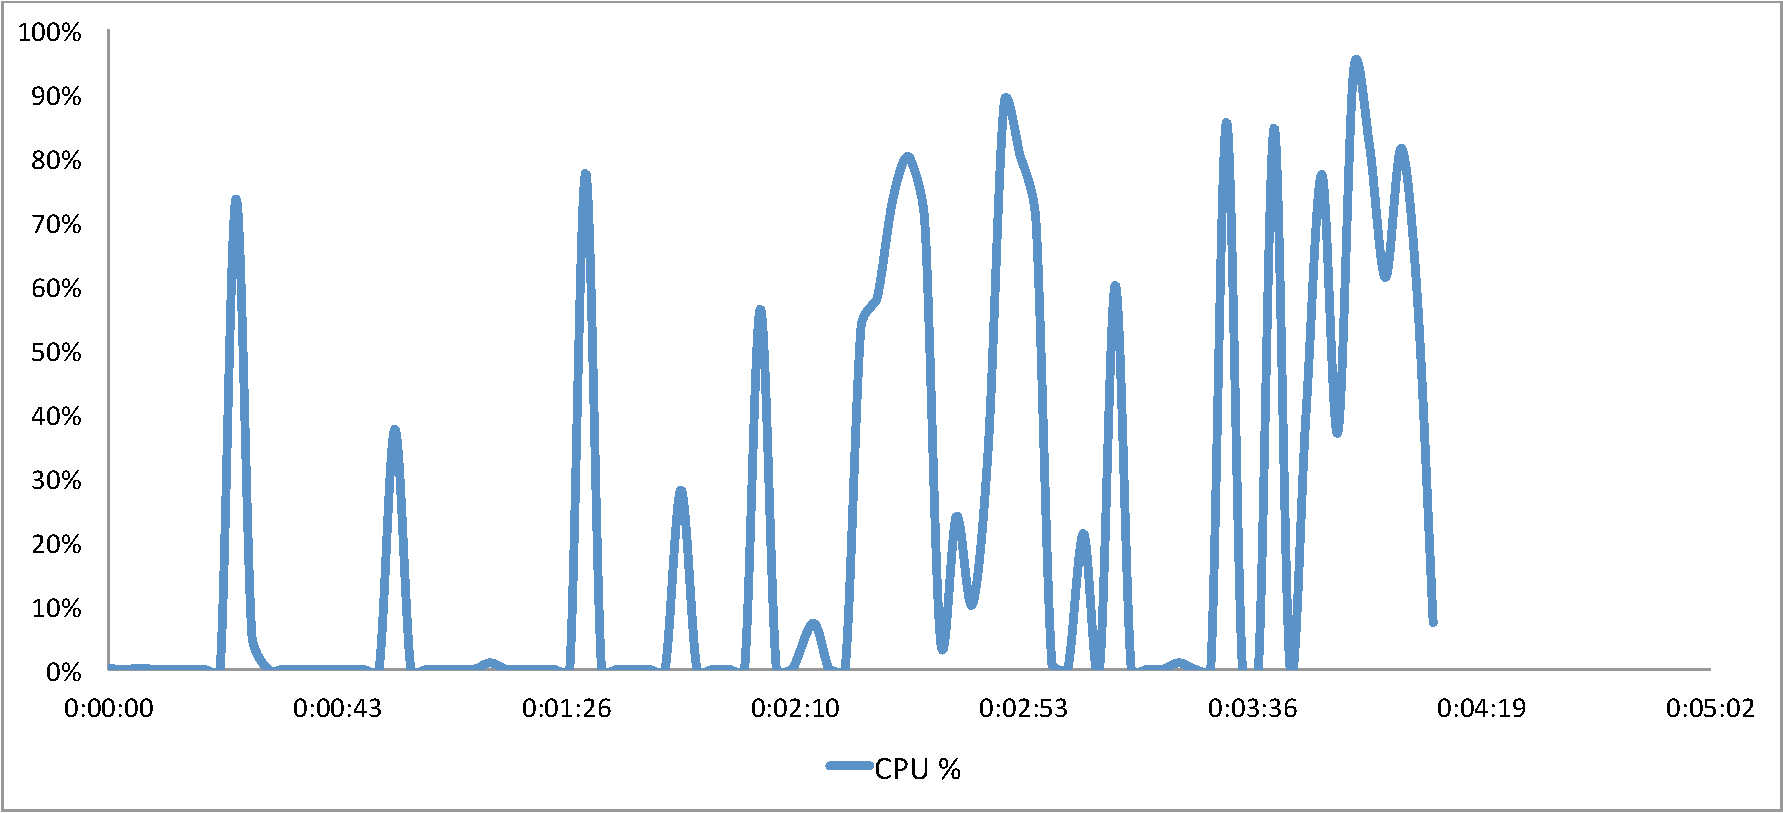
\includegraphics[width =\textwidth] {results/hand_new_cpu.pdf}
	\label{fig:hand_new_cpu}
}
\subfigure[b][Memory Usage]{
	\centering
	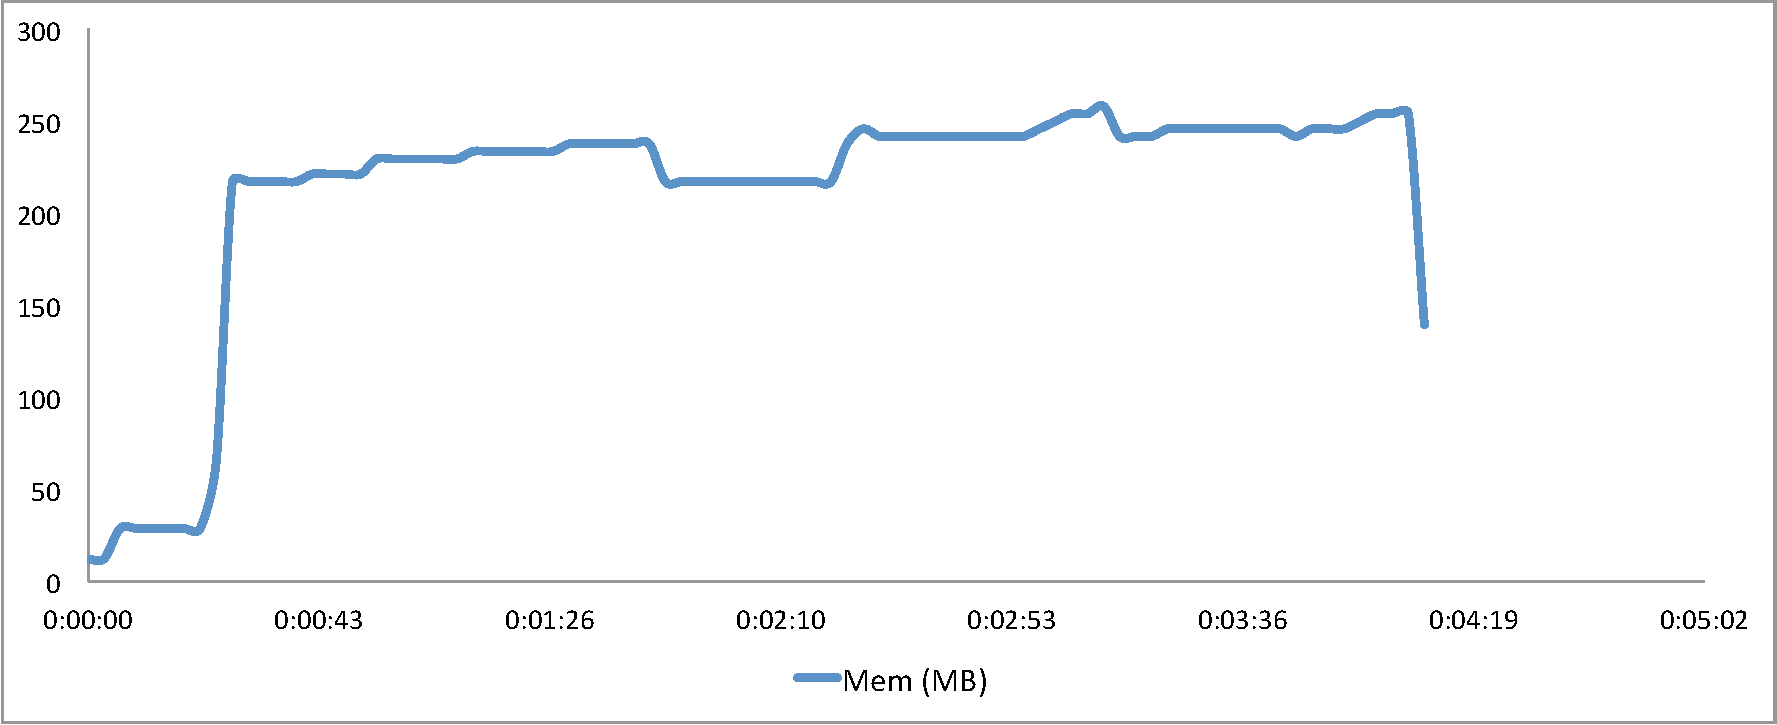
\includegraphics[width =\textwidth] {results/hand_new_mem.pdf}
	\label{fig:hand_new_mem}
}
\label{fig:hand_new_cpu_mem}
\caption{CPU and Memory Usage of Experiment on model "hand\_new"}
\end{figure}
We use model "hand\_new" for our Memory/CPU Usage experiment. The results are showed in \FGp{fig:hand_new_cpu_mem}. \FG{fig:hand_new_cpu} illustrates the CPU usage from the beginning of streaming. During the experiment the model is rotated and zoomed in for different viewing angle and scale. We can see from it that there are a climax of CPU usage between each idle time, which is the effects of each server processing between two viewing parameter synchronization request from server. \FG{fig:hand_new_cpu_mem} shows the memory usage. It shows that the server's memory consumption is quite steady during streaming. 


\subsubsection{Visual Quality}
\label{section:clientvisualquality}
\begin{figure}
\centering
\subfigure[b][]{
	\centering
	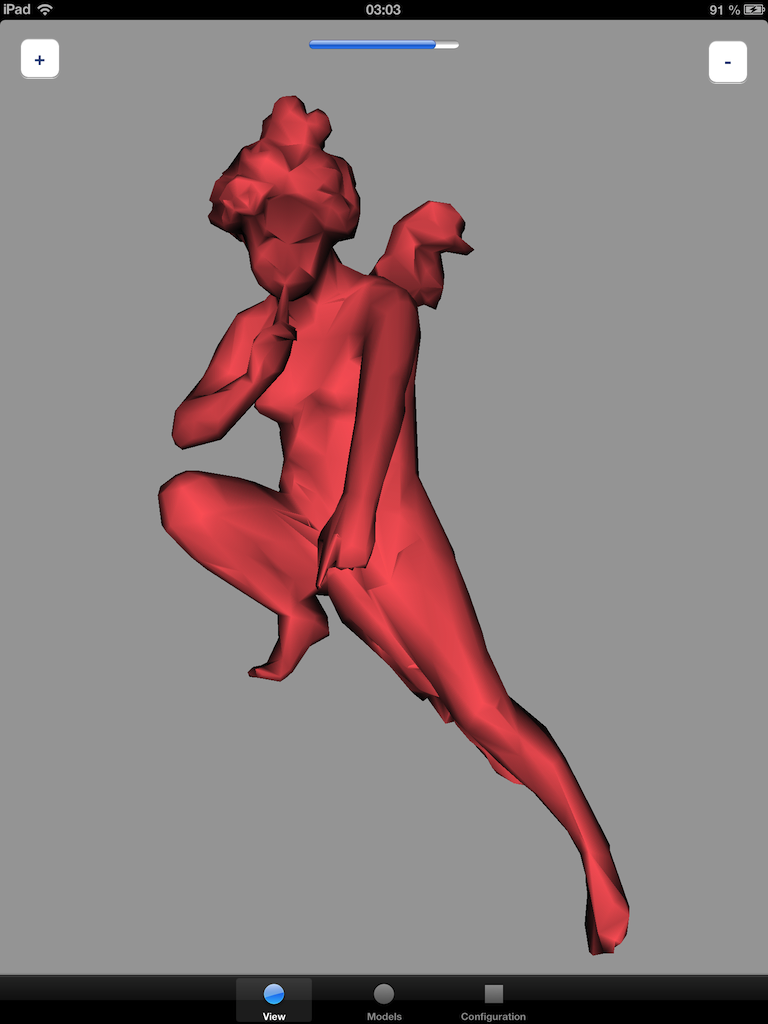
\includegraphics[width =0.45\textwidth] {results/030330.png}
	\label{fig:angel_visual_effects_1}
}
\hfill
\subfigure[b][]{
	\centering
	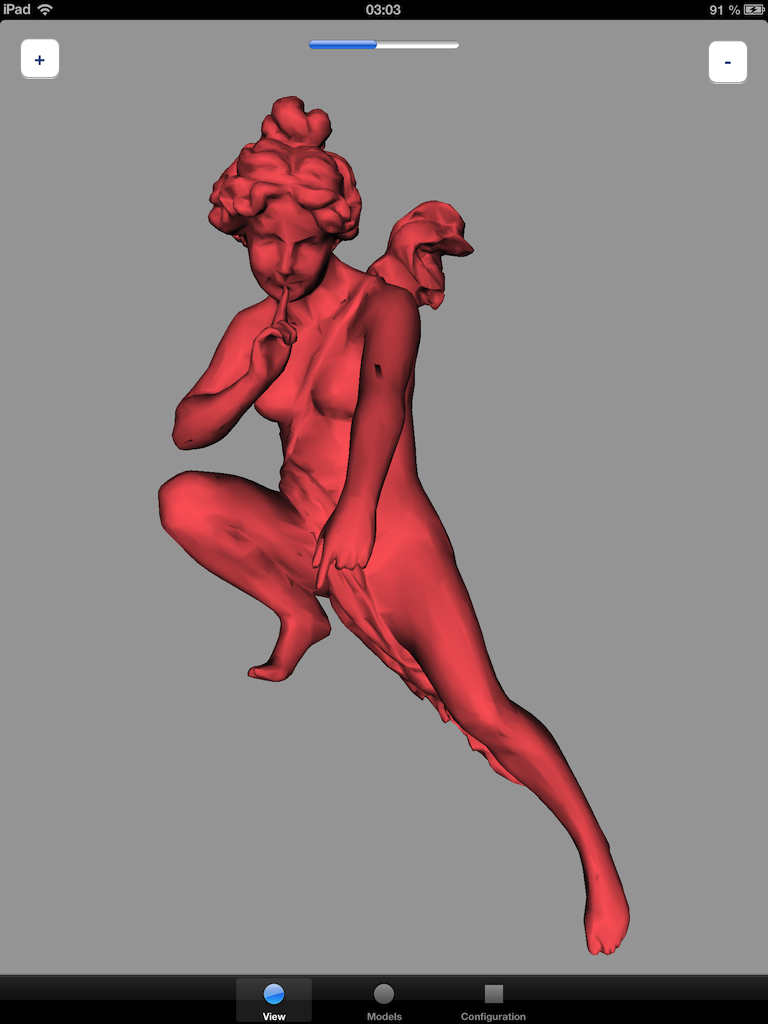
\includegraphics[width =0.45\textwidth] {results/030333.png}
	\label{fig:angel_visual_effects_2}
}

\subfigure[b][]{
	\centering
	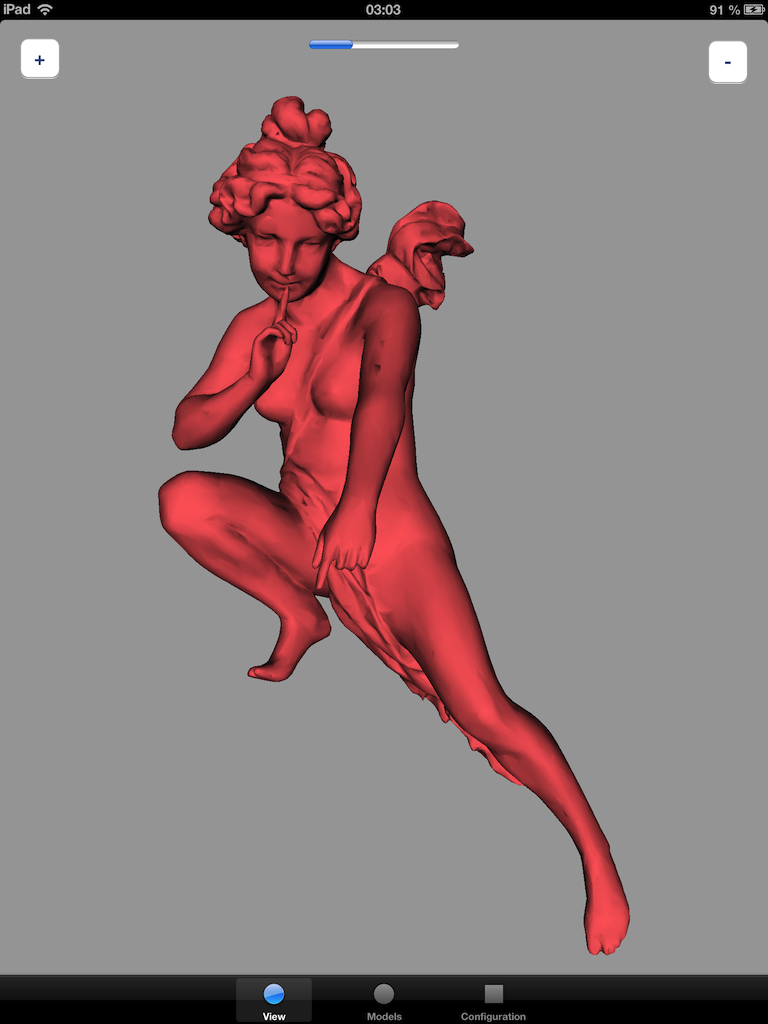
\includegraphics[width =0.45\textwidth] {results/030337.png}
	\label{fig:angel_visual_effects_3}
}
\hfill
\subfigure[b][]{
	\centering
	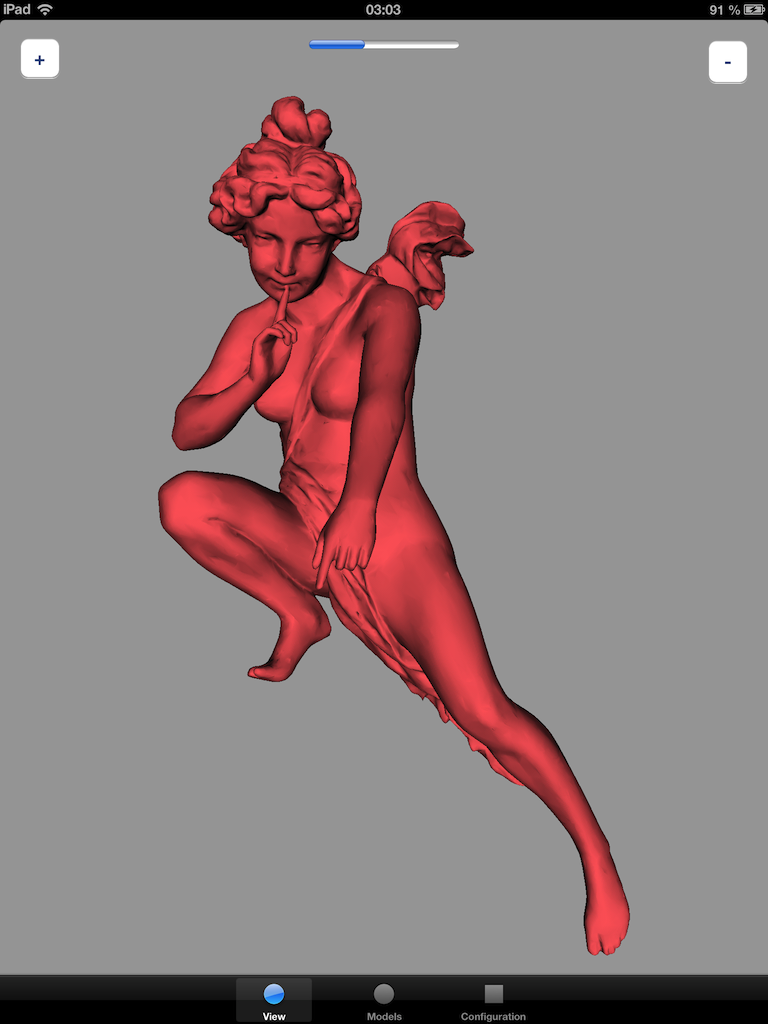
\includegraphics[width =0.45\textwidth] {results/030348.png}
	\label{fig:angel_visual_effects_4}
}

\label{fig:angel_visual_effects}
\caption{Visual Effects of Model "angel"}

\end{figure}

\begin{figure}
\centering

\subfigure[b][]{
	\centering
	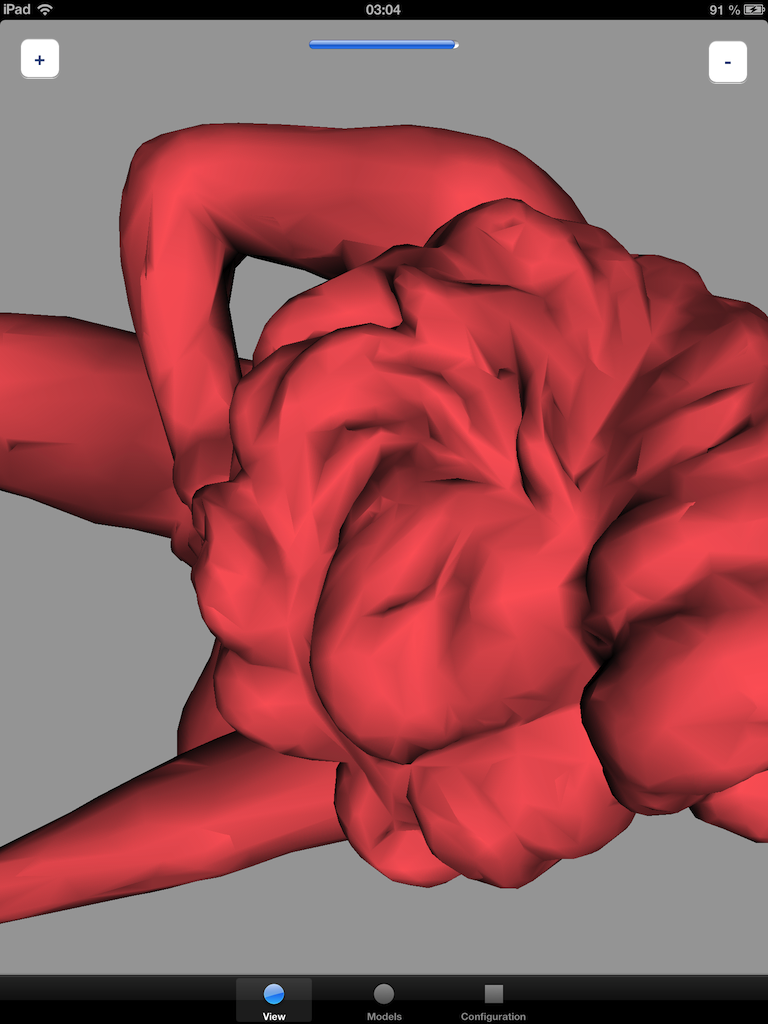
\includegraphics[width =0.45\textwidth] {results/030442.png}
	\label{fig:angel_visual_effects_hair2}
}
\hfill
\subfigure[b][]{
	\centering
	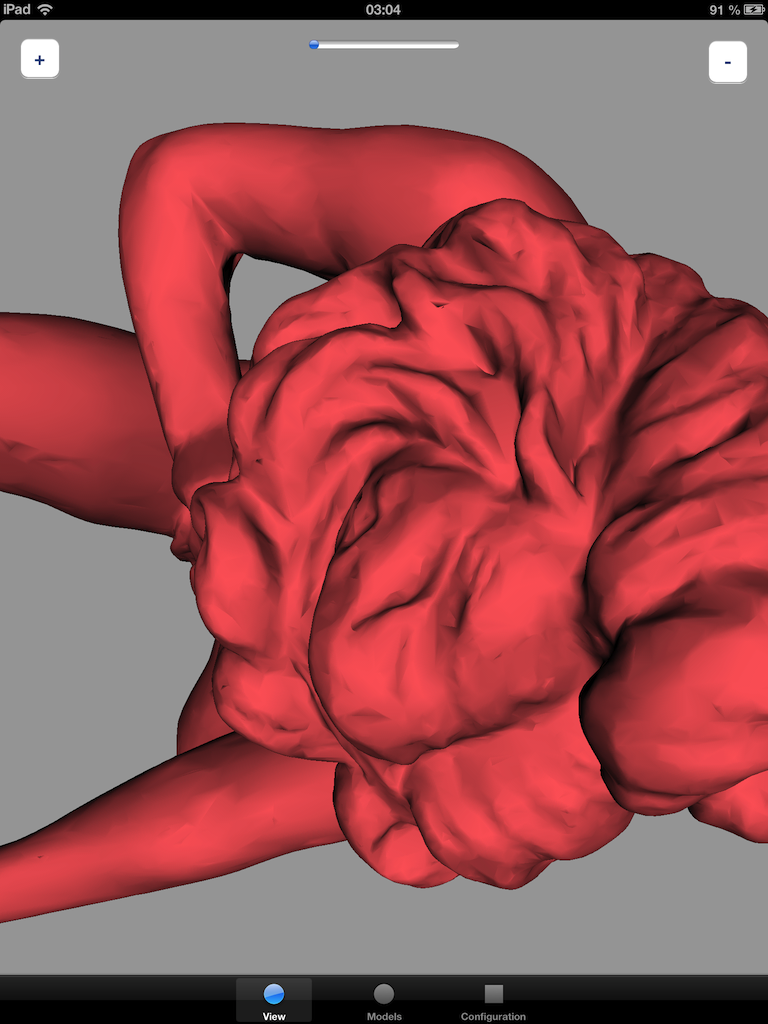
\includegraphics[width =0.45\textwidth] {results/030459.png}
	\label{fig:angel_visual_effects_hair4}
}

\subfigure[b][]{
	\centering
	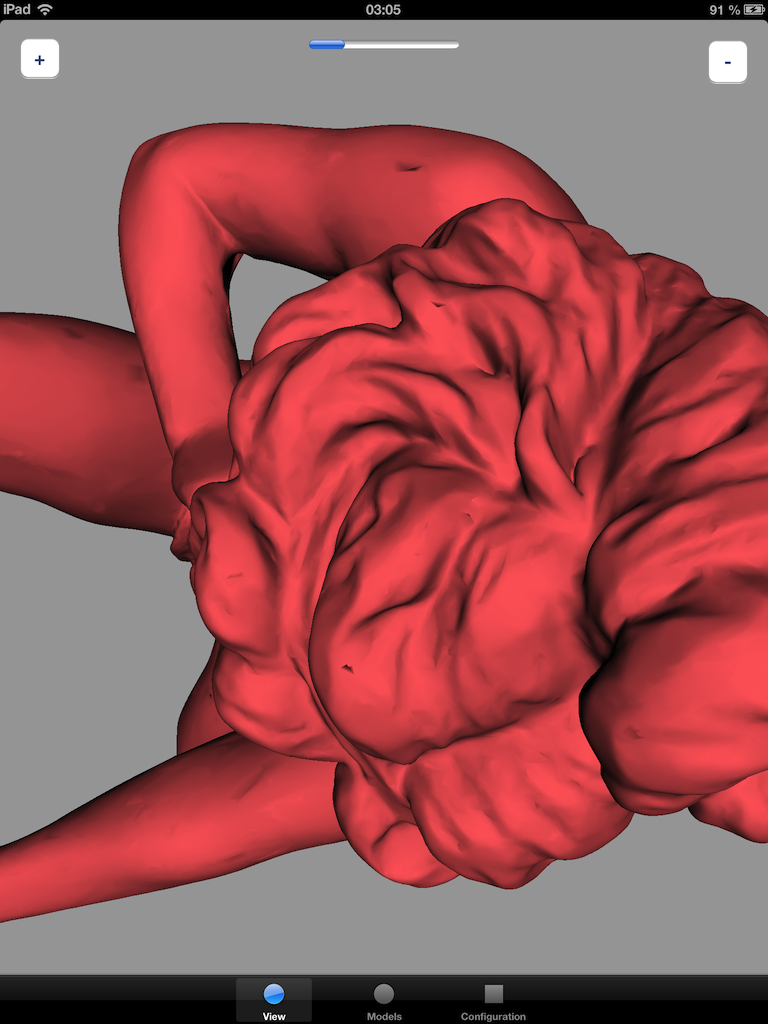
\includegraphics[width =0.45\textwidth] {results/030519.png}
	\label{fig:angel_visual_effects_hair6}
}
\hfill
\subfigure[b][]{
	\centering
	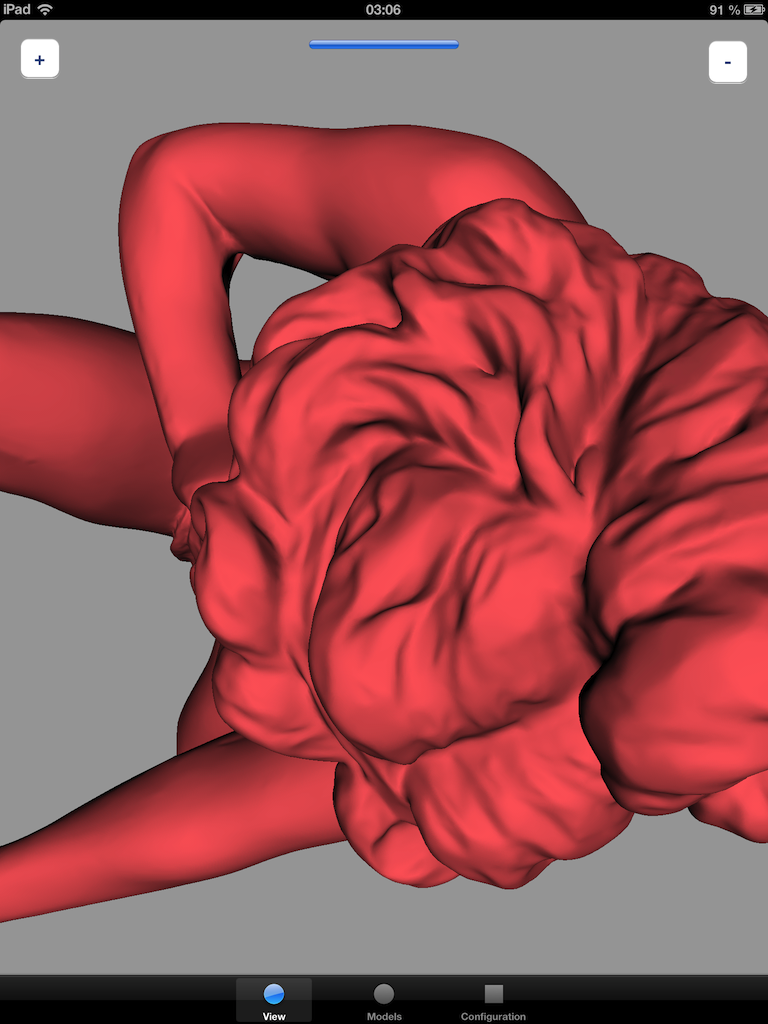
\includegraphics[width =0.45\textwidth] {results/030607.png}
	\label{fig:angel_visual_effects_hair8}
}

\label{fig:angel_visual_effects_hair}
\caption{Visual Effects of Model "angel"'s "hair"}
\end{figure}
When the client side start to stream a mesh, it will be viewed on the client screen and refined on-the-fly, which means it can be seen as a refinement animation. Therefore we choose to illustrate this process in a sequence of screen shots using the model "angel". 







\subsection{Server Rendering Evaluation}
\label{section:servereva}
\begin{figure}
\centering
\subfigure[b][Size of Data Transfer. For each viewing param sync request, an image will be rendered in corresponding LOD and transmitted to client. We can see that the time of server side refinement and rendering is quite stable and the accumulative size of data transmitted are linearly increasing, as expected.]{
	\centering
	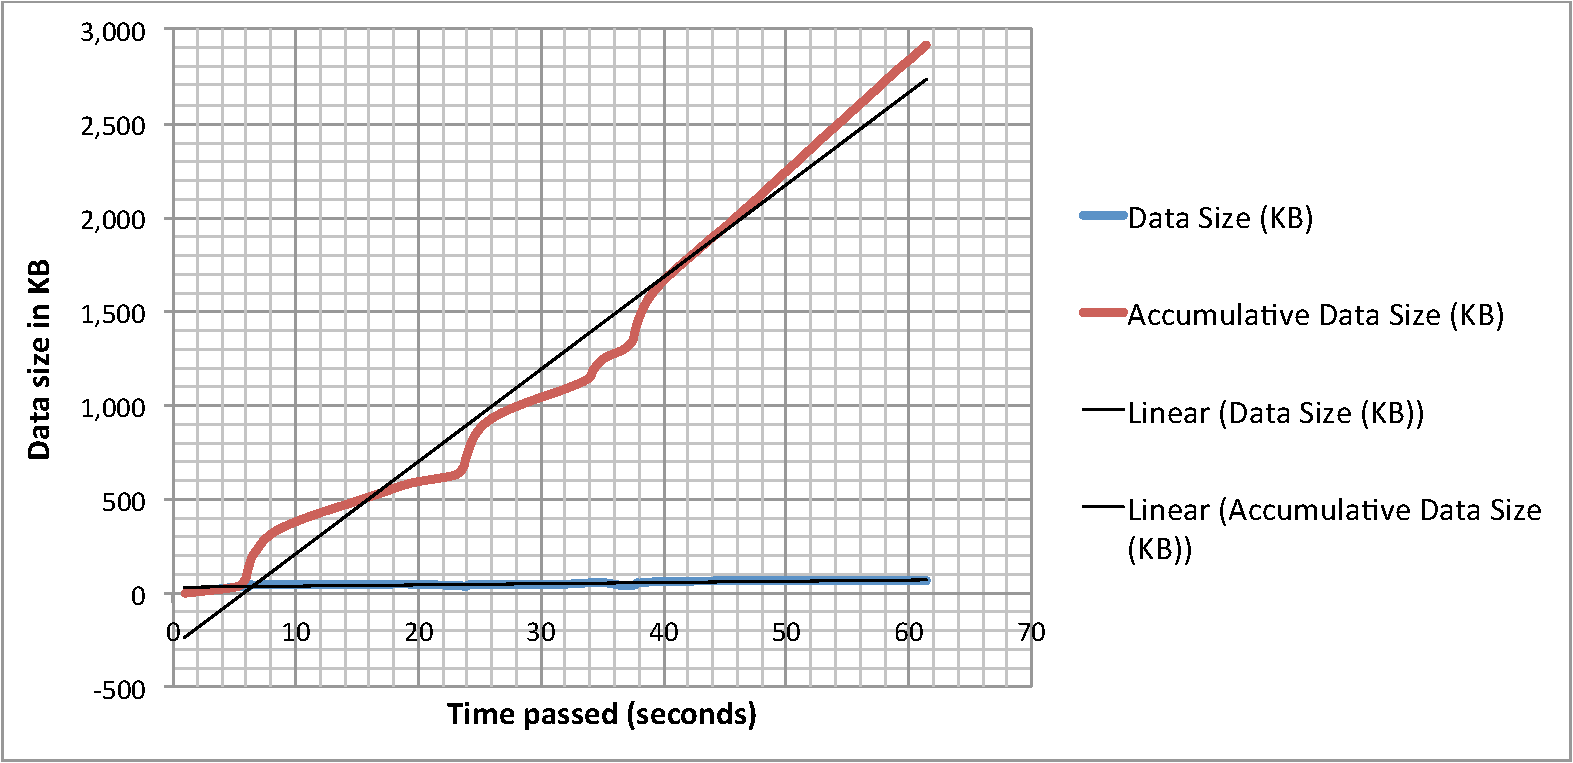
\includegraphics[width =\textwidth] {results/hapy_vrip_trans_datasize.pdf}
	\label{fig:hapy_vrip_svr_data_trans_datasize}
}
\subfigure[b][Num. of active vertices and faces of the server-hold model during streaming. The low points in the middle of the graph indicates the user is changing view and unnecessary edges are collapsed, unnecessary vertices are eliminated.]{
	\centering
	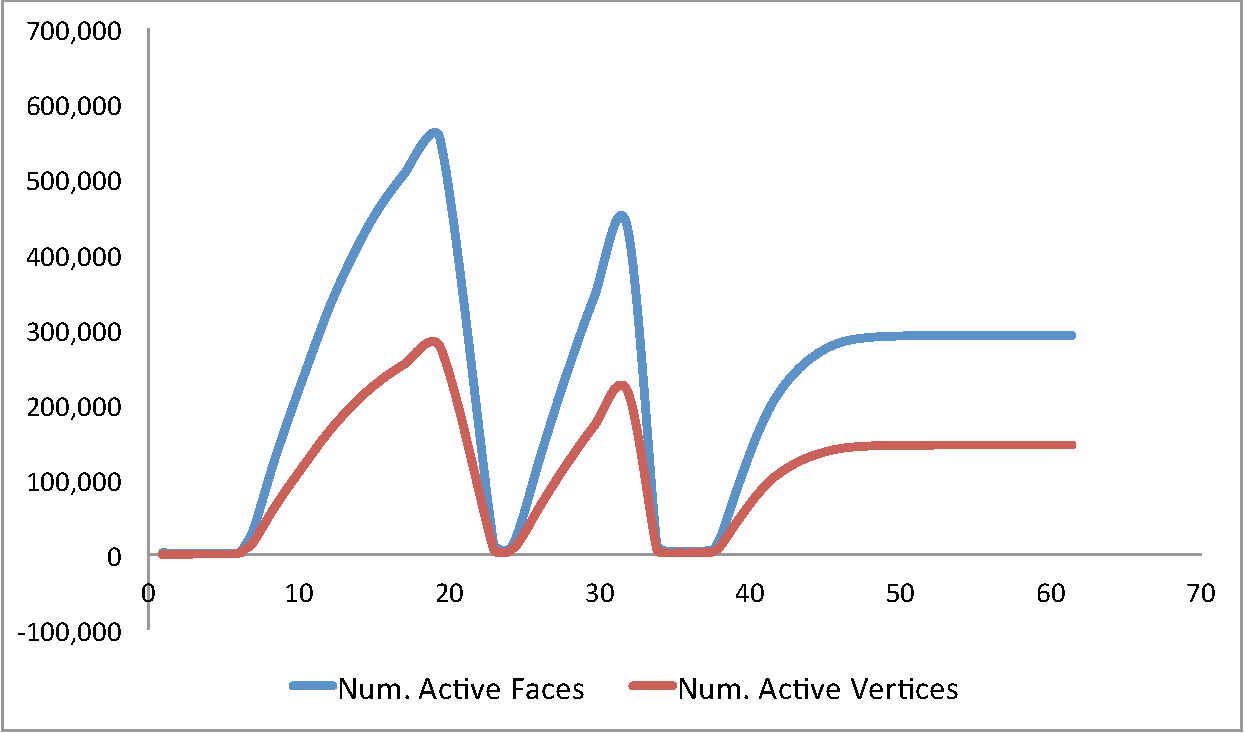
\includegraphics[width =\textwidth] {results/hapy_vrip_vfront_over_time.pdf}
	\label{fig:hapy_vrip_svr_data_trans_active_faces_vertices}
}
\label{fig:hapy_vrip_svr_data_trans}
\caption{Server Rendering Data Transmission Statistics of model "hapy\_vrip"}
\end{figure}
The server rendering evaluation experiments are performed on the models listed in \TA{table:modelsserverrendering}.

\subsubsection{Transmission Performance}
\label{section:servertransperf}
Since in the server rendering situation, both the refinement and rendering is done by the server, the definition of elapsed time becomes: $Time_{refinement}+Time_{rendering}+Time_{transmission}$. We choose the model "hapy\_vrip" for experiment. Details see \FGp{fig:hapy_vrip_svr_data_trans}. We can see that the server rendering of big meshes is quite fast. 



\subsubsection{Visual Quality}
\label{section:servervisualquality}

\begin{figure}
\centering
\subfigure[b][Visual Effects at low LOD level]{
	\centering
	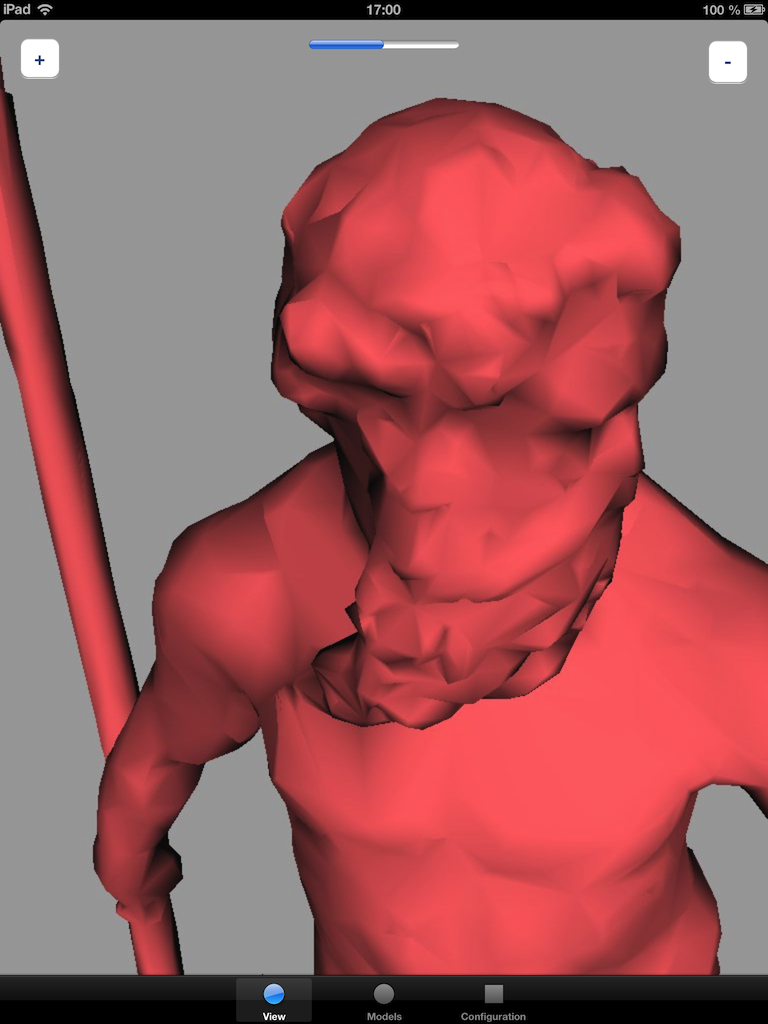
\includegraphics[width =0.3\textwidth] {results/170035.png}
	\label{fig:neptune_serverrendering_visual_effects1}
}
\hfill
\subfigure[b][Visual Effects at medium LOD level]{
	\centering
	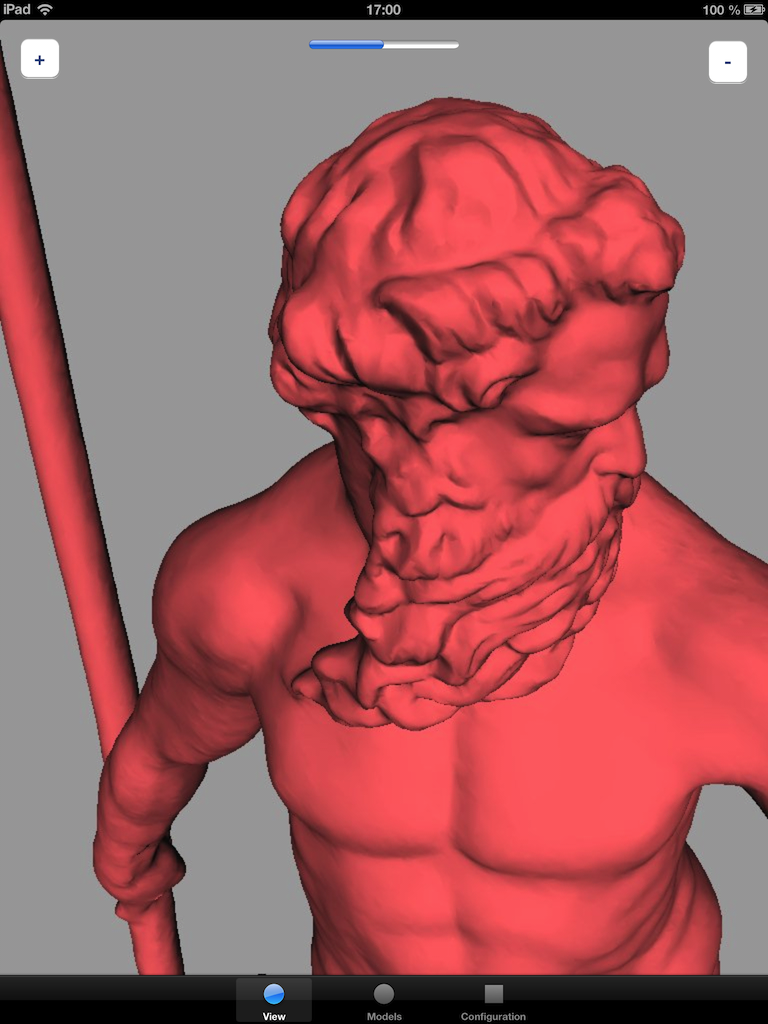
\includegraphics[width =0.3\textwidth] {results/170038.png}
	\label{fig:neptune_serverrendering_visual_effects2}
}
\hfill
\subfigure[b][Visual Effects at high LOD level]{
	\centering
	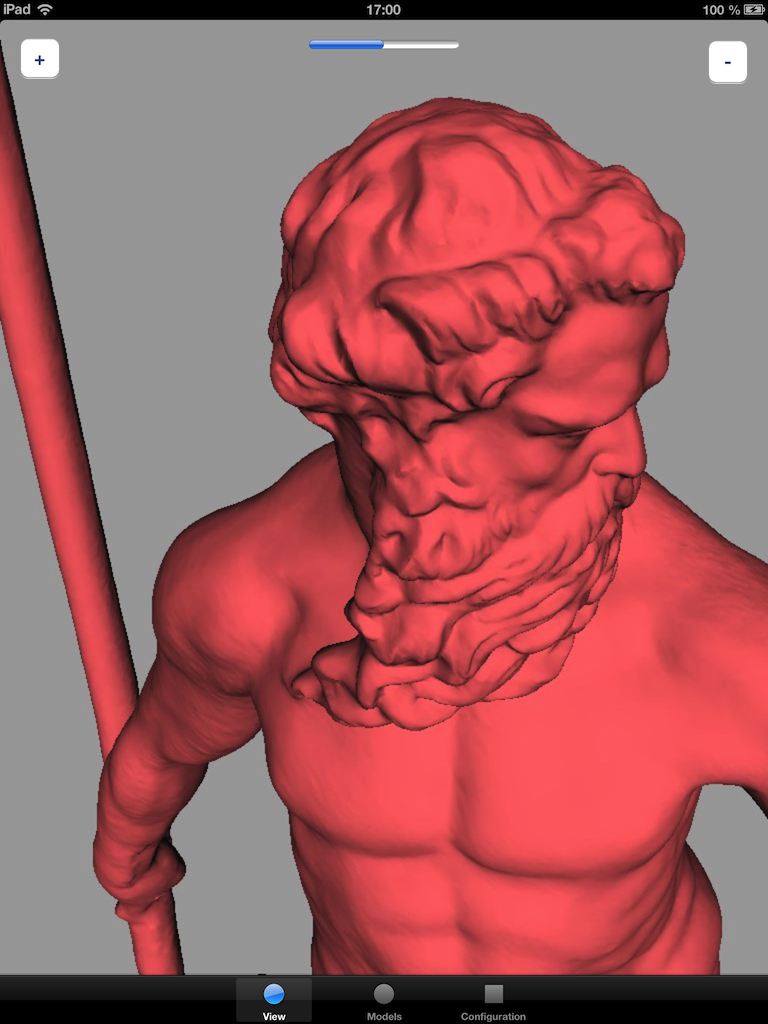
\includegraphics[width =0.3\textwidth] {results/170041.png}
	\label{fig:neptune_serverrendering_visual_effects3}
}

\label{fig:neptune_serverrendering_visual_effects}
\caption{Server Rendering Visual Effects of model "803\_neptune\_4Mtriangles\_manifold" with 4M triangles}
\end{figure}

Similar to \SC{section:clientvisualquality}, in this section we will illustrate some screen shots to show the visual quality of server rendering streaming (See \FGp{fig:neptune_serverrendering_visual_effects}). It can be found that there is significant different between \FG{fig:neptune_serverrendering_visual_effects1} and \FG{fig:neptune_serverrendering_visual_effects2}, while \FG{fig:neptune_serverrendering_visual_effects2} and \FG{fig:neptune_serverrendering_visual_effects3} looks almost the same. This is because when model's LOD reaches a certain high level, the triangles reconstructed could even be smaller than a pixel on screen, thus making it looks no difference compared with lower LOD level. 

\section{Discussion}
\label{section:results:discussion}
%\TODO{Discussion of test results. }
In the previous paragraphs, we have illustrated the result of experiment on our framework. It can be found that for both client and server rendering scenario, our framework is able to provide stable functionality of view-dependent progressive mesh streaming with high visual quality and performance. \\

In the scenario of client rendering, the performance bottleneck is mainly the client side since the model will finally reconstructed and rendered by the client and meanwhile the client has to support interruptible user interaction during refinement and rendering. On the other hand, in the scenario of server rendering, performance burden on client is relatively light and the main performance bottleneck is in the server side. The server needs to do almost every thing including refinement and rendering. And the client just have to show the rendered images from server. \\ 


%Picture
%\noindent
%\begin{minipage}{\linewidth}
%\makebox[\linewidth]{%
%\includegraphics[width=1.0\textwidth]{images/morphable.pdf}}
%\captionof{figure}{MorphableUI generates user-tailored interfaces for arbitrary applications in arbitrary environments. Users are able to use all available devices to control as many applications as needed. User behavior is analyzed by the system to increase the user experience.}% only if needed
%\label{fig:morphable}
%\bigskip
%\end{minipage}


